%Input preamble
\documentclass[11pt]{article}

% colors
\usepackage[table]{xcolor}
\definecolor{maroon}{RGB}{153,0,18}
\definecolor{lime}{RGB}{190,213,88}
\definecolor{sand}{RGB}{217,202,179}
\definecolor{fire}{RGB}{144,50,61}
\definecolor{brick}{RGB}{94,11,21}
\definecolor{olive}{RGB}{117,109,84}
\definecolor{lavpink}{RGB}{172,123,132}
\definecolor{darkpurp}{RGB}{49,10,49}
\definecolor{salmon}{RGB}{204,90,113}
\definecolor{mauve}{RGB}{94,73,85}
\definecolor{greyblue}{RGB}{125,132,145}
\definecolor{greypurp}{RGB}{68,56,80}
\definecolor{brightpurp}{RGB}{96,20,255}

% packages (please add in alphabetical order)
\usepackage{adjustbox}
\usepackage{amsfonts}
\usepackage{amsmath}
\usepackage{amssymb}
\usepackage{array}
\usepackage{bm}
\usepackage{booktabs}
\usepackage{caption}
\usepackage{epstopdf}
\usepackage{float}
\usepackage[margin=1in]{geometry}
\usepackage{graphicx}
\usepackage[colorlinks=true, linkcolor=brightpurp, citecolor=brightpurp, urlcolor=salmon]{hyperref}
\usepackage{lipsum}
\usepackage{longtable}
\usepackage{mathtools}
\usepackage{multirow}
\usepackage{natbib}
\usepackage{rotating}
\usepackage{setspace}
\usepackage{subcaption}
%\usepackage{threeparttable}
\usepackage{threeparttablex}
\usepackage{xr}
\usepackage[printwatermark]{xwatermark}


\newcolumntype{L}[1]{>{\raggedright\let\newline\\\arraybackslash\hspace{0pt}}m{#1}}
\newcolumntype{C}[1]{>{\centering\let\newline\\\arraybackslash\hspace{0pt}}m{#1}}
\newcolumntype{R}[1]{>{\raggedleft\let\newline\\\arraybackslash\hspace{0pt}}m{#1}}

% commands
\newcommand{\mr}{\multirow}
\newcommand{\mc}{\multicolumn}




\begin{document}


\begin{sidewaysfigure}[!htpb]
\centering
\caption{Gender and Socioeconomic Disadvantage in the Control Group} 
\begin{subfigure}[h]{0.45\textwidth}
	\centering
	\caption{Take-up of Alternatives by Gender} 
	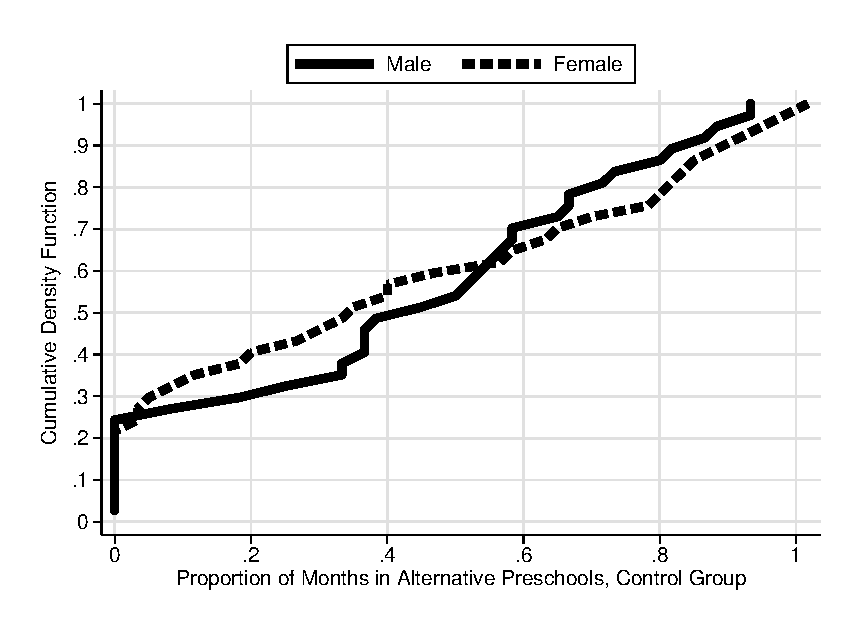
\includegraphics[width=\textwidth]{output/abccare_controlcontamination_boysgirls}
\end{subfigure}%
\begin{subfigure}[h]{0.45\textwidth}
	\centering
	\caption{Socioeconomic Disadvantage by Gender} 
	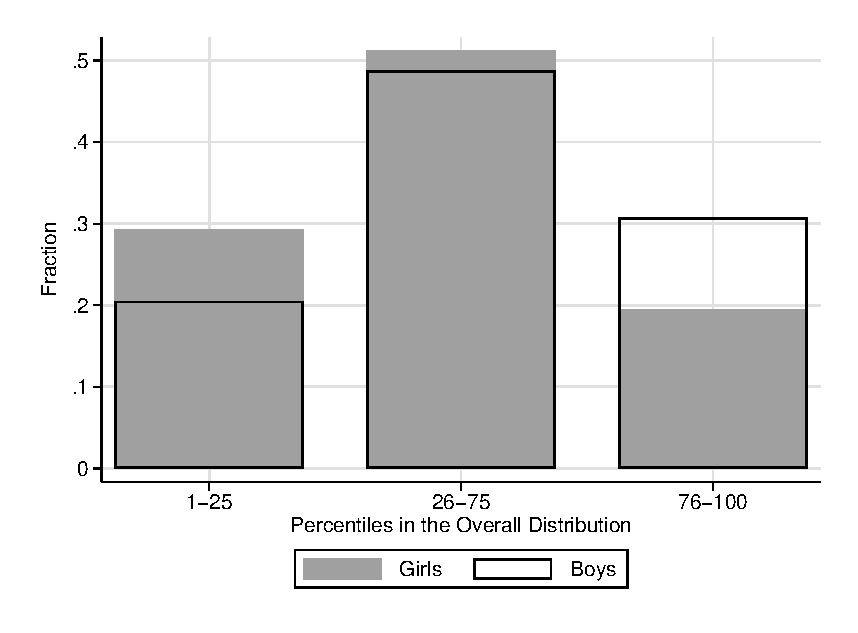
\includegraphics[width=\textwidth]{output/factorbase_girlsboyscompare}
\end{subfigure}
\begin{subfigure}[h]{0.45\textwidth}
	\centering
	\caption{Take-up of Alternatives by Disadvantage, Girls} 
	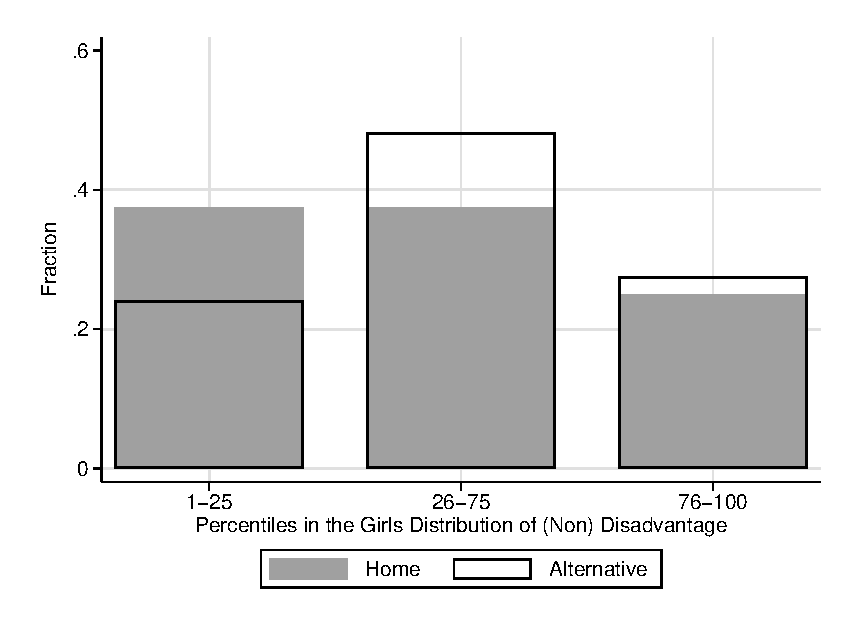
\includegraphics[width=\textwidth]{output/factorbase_wgirlscompare}
\end{subfigure}%
\begin{subfigure}[h]{0.45\textwidth}
	\centering
	\caption{Take-up of Alternatives by Disadvantage, Boys} 
	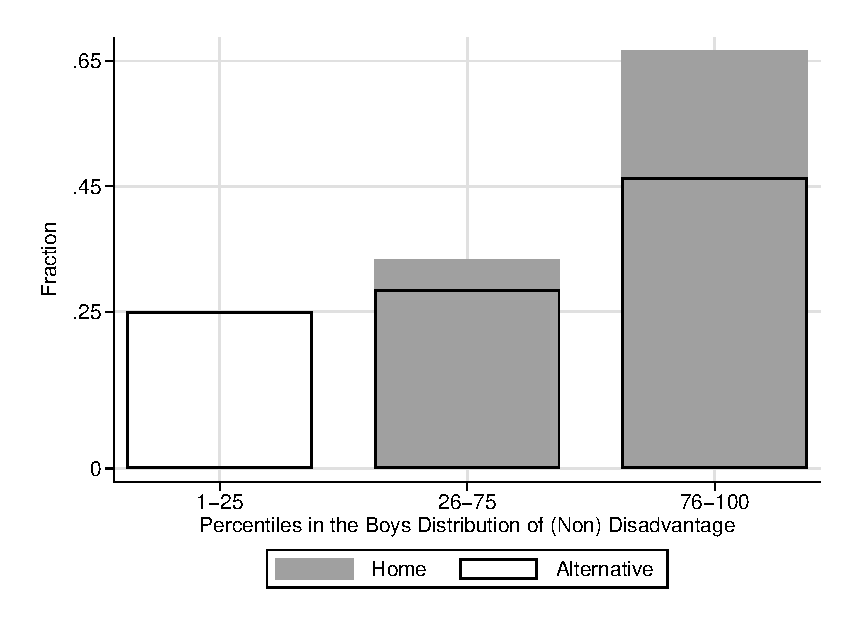
\includegraphics[width=\textwidth]{output/factorbase_wboyscompare}
\end{subfigure}
\footnotesize
\justify
\textbf{Note:} Panel (a) .
\end{sidewaysfigure}





\end{document}


